% Software Engineering & System Simulation
% Interview deck for Delta Electronics software roles and NVIDIA software /
% system-software roles. November 6, 2026.
%
% Engine: pdfLaTeX (same as NV-Testing). 16:9 Beamer.
% Diagrams are TikZ in this file. Do not add measured results, incidents,
% or a claim that the LLM simulator is already integrated.
%
% NeoPower scope follows the presenter's finalized explanation.
% Existing Beamer identity and useful architecture diagrams are preserved.
%
% Slide sequence:
%  1 Cover
%  2 Education & Professional Experience
%  3 NeoPower architecture
%  4 NeoPower scenario simulation
%  5 NeoPower testing and reliability
%  6 Cross-data-center heterogeneous GPU serving
%  7 System-level simulation methodology
%  8 Thank you

\documentclass[aspectratio=169,10pt]{beamer}
\usepackage[english]{babel}
\usepackage[utf8]{inputenc}
\usepackage[T1]{fontenc}
\usepackage{lmodern}
\usepackage{amsmath,amssymb}
\usepackage{graphicx}
\usepackage{xcolor}
\usepackage{tikz}
\usetikzlibrary{arrows.meta,positioning,calc,fit,backgrounds}
\usepackage{hyperref}
\graphicspath{{./}{figures/}}
\hypersetup{hidelinks}

% --------- Madrid-inspired identity, matched to NV-Testing ---------
\usetheme{Madrid}
\usecolortheme{default}
\definecolor{Ink}{HTML}{243748}
\definecolor{Muted}{HTML}{667B8B}
\definecolor{Accent}{HTML}{347E74}
\definecolor{AccentBlue}{HTML}{507DAD}
\definecolor{SoftMint}{HTML}{E6F4EE}
\definecolor{SoftBlue}{HTML}{E9F2F9}
\definecolor{SoftLilac}{HTML}{F1EEF8}
\definecolor{Paper}{HTML}{FBFCFE}
\definecolor{Divider}{HTML}{D8E4EB}
\setbeamercolor{background canvas}{bg=Paper}
\setbeamercolor{normal text}{fg=Ink}
\setbeamercolor{structure}{fg=Accent}
\setbeamercolor{frametitle}{fg=Ink,bg=SoftBlue}
\setbeamercolor{title}{fg=Ink}
\setbeamercolor{subtitle}{fg=Muted}
\setbeamercolor{block title}{fg=Ink,bg=SoftBlue}
\setbeamercolor{block body}{fg=Ink,bg=white}
\setbeamercolor{item}{fg=Accent}
\setbeamercolor{footline}{fg=Muted,bg=Paper}
\setbeamercolor{panelblue}{fg=Ink,bg=SoftBlue!60}
\setbeamercolor{panelmint}{fg=Ink,bg=SoftMint!72}
\setbeamercolor{panellilac}{fg=Ink,bg=SoftLilac!76}
\setbeamercolor{panelwhite}{fg=Ink,bg=white}
\setbeamerfont{frametitle}{size=\Large,series=\bfseries}
\setbeamerfont{footline}{size=\tiny}
\setbeamertemplate{headline}{}
\setbeamertemplate{navigation symbols}{}
\setbeamertemplate{blocks}[rounded][shadow=false]
\setbeamertemplate{itemize items}[circle]
\setbeamertemplate{footline}{%
  \leavevmode\hbox{%
    \begin{beamercolorbox}[wd=\paperwidth,ht=.30cm,dp=.16cm,rightskip=.60cm plus 1fil]{footline}%
      \hfill\insertframenumber\,/\,\inserttotalframenumber
    \end{beamercolorbox}}%
}
\setbeamertemplate{frametitle}{%
  \nointerlineskip
  \begin{beamercolorbox}[wd=\paperwidth,ht=.77cm,dp=.18cm,leftskip=.64cm]{frametitle}%
    \usebeamerfont{frametitle}\insertframetitle
  \end{beamercolorbox}%
}

% --------- Reusable text components ---------
\newcommand{\smalllabel}[1]{{\scriptsize\bfseries\color{Accent}\MakeUppercase{#1}}}
\newcommand{\takeaway}[1]{%
  \begin{beamercolorbox}[rounded=true,sep=0.12cm,wd=\linewidth]{block title}%
    \raggedright\strut\textbf{#1}\strut
  \end{beamercolorbox}%
}
% Diagram styles. HBM is blue, HBF is mint, hybrid cells are split.
% Hybrid cell geometry must match memcell: text width 2.48cm, inner sep 3pt,
% minimum height 1.26cm.
\newcommand{\hybridcell}[3]{%
  \begin{scope}
    \clip[rounded corners=3pt] (#1-1.35,#2-0.63) rectangle (#1+1.35,#2+0.63);
    \fill[SoftBlue!88] (#1-1.35,#2-0.63) rectangle (#1,#2+0.63);
    \fill[SoftMint] (#1,#2-0.63) rectangle (#1+1.35,#2+0.63);
  \end{scope}
  \draw[Ink!30, rounded corners=3pt, line width=0.7pt]
    (#1-1.35,#2-0.63) rectangle (#1+1.35,#2+0.63);
  \node[align=center, font=\small, text width=2.30cm] at (#1,#2) {#3};
}
\tikzset{
  svc/.style={rounded corners=3pt, align=center, font=\small,
    inner sep=3.5pt, line width=0.75pt},
  fe/.style={svc, draw=AccentBlue!65, fill=SoftBlue!75,
    text width=2.45cm, minimum height=1.08cm},
  be/.style={svc, draw=Accent!80, fill=SoftMint,
    text width=3.35cm, minimum height=1.08cm},
  store/.style={svc, draw=AccentBlue!45, fill=white,
    text width=2.55cm, minimum height=1.28cm},
  extbox/.style={svc, draw=AccentBlue!55, fill=SoftLilac,
    text width=2.75cm, minimum height=1.08cm},
  scen/.style={rounded corners=3pt, align=center, font=\small,
    text width=2.85cm, minimum height=2.02cm, inner sep=3.5pt, line width=0.75pt,
    execute at begin node={\hyphenpenalty=10000\exhyphenpenalty=10000\sloppy}},
  flowstep/.style={draw=Accent!65, fill=white, rounded corners=3pt,
    minimum height=0.92cm, text width=2.20cm, align=center,
    inner sep=3pt, font=\small, line width=0.75pt},
  memcell/.style={rounded corners=3pt, align=center, font=\small,
    text width=2.48cm, minimum height=1.26cm, inner sep=3pt, line width=0.7pt},
  demand/.style={rounded corners=3pt, align=center, font=\small,
    text width=3.05cm, minimum height=0.68cm, inner sep=2pt, line width=0.7pt},
  srcbox/.style={rounded corners=3pt, align=flush left, font=\small,
    text width=3.25cm, minimum height=1.78cm, inner sep=4pt, line width=0.75pt},
  hubbox/.style={rounded corners=3pt, align=flush left, font=\small,
    text width=3.85cm, minimum height=3.72cm, inner sep=5pt, line width=0.8pt},
  method/.style={rounded corners=3pt, align=center, font=\small\bfseries,
    minimum height=0.72cm, text width=2.85cm, inner sep=3pt}
}

\title[Software Engineering]{Software Engineering \& System Simulation}
\subtitle{Production Software Development / GPU LLM Serving Research}
\author{Yu-Jui Liang}
\institute{National Taiwan University}
\date{}

\begin{document}

% ============================================================
% SLIDE 1 - Cover
% ============================================================
{\setbeamertemplate{footline}{}
\begin{frame}[plain]
  \vspace*{0.82cm}
  {\normalsize\bfseries\color{Accent}SOFTWARE ENGINEER INTERVIEW}\par
  \vspace{0.48cm}
  {\raggedright\fontsize{20}{24}\selectfont\bfseries\color{Ink}
    Software Engineering \& System Simulation\par}
  \vspace{0.34cm}
  {\color{Muted}\fontsize{11}{14}\selectfont Production Software Development \quad$\cdot$\quad GPU LLM Serving Research\par}
  \vspace{0.72cm}
  {\large\bfseries Yu-Jui Liang}\par
  \vfill
\end{frame}}

% ============================================================
% SLIDE 2 - Education & Professional Experience
% Copied from NV-Testing slide 2 for consistent education and career history.
% ============================================================
\begin{frame}{Education \& Professional Experience}
  \vspace{0.05cm}

  \begin{columns}[T,onlytextwidth]

    % ----- Education -----
    \begin{column}{0.49\textwidth}
      \begin{beamercolorbox}[
        rounded=true,sep=0.20cm,wd=\linewidth
      ]{panelblue}

        {\large\bfseries\color{AccentBlue}
          Education}\par
        \vspace{0.24cm}

        {\normalsize\bfseries
          National Taiwan University}\par
        \vspace{0.06cm}
        {\normalsize
          M.S. Candidate, Data Science
          Master's Degree Program}\par
        \vspace{0.05cm}
        {\small\color{Muted}
          Expected Graduation: June 2027}\par

        \vspace{0.26cm}
        {\color{Divider}\rule{0.92\linewidth}{0.4pt}}
        \vspace{0.19cm}

        {\normalsize\bfseries
          National Chengchi University}\par
        \vspace{0.06cm}
        {\normalsize
          B.S. in Computer Science}\par
        {\normalsize
          Double Major in Electronic Physics}\par
        \vspace{0.05cm}
        {\small\color{Muted}
          Sep. 2021 -- Jun. 2025}\par

      \end{beamercolorbox}
    \end{column}

    % ----- Professional Experience -----
    \begin{column}{0.49\textwidth}
      \begin{beamercolorbox}[
        rounded=true,sep=0.20cm,wd=\linewidth
      ]{panelmint}

        {\large\bfseries\color{Accent}
          Professional Experience}\par
        \vspace{0.24cm}

        {\normalsize\bfseries
          AIMobile Co., Ltd.}\par
        {\small\color{Muted}
          Inventec Group}\par
        \vspace{0.06cm}
        {\normalsize
          Contract Software Engineer}\par
        \vspace{0.05cm}
        {\small\color{Muted}
          Apr. 2025 -- Jul. 2025}\par

        \vspace{0.26cm}
        {\color{Divider}\rule{0.92\linewidth}{0.4pt}}
        \vspace{0.19cm}

        {\normalsize\bfseries
          Neopower Technologies\\Co., Ltd.}\par
        \vspace{0.06cm}
        {\normalsize
          Contract Software Engineer}\par
        \vspace{0.05cm}
        {\small\color{Muted}
          Jun. 2023 -- Mar. 2025}\par

      \end{beamercolorbox}
    \end{column}

  \end{columns}
\end{frame}

% ============================================================
% SLIDE 3 - NeoPower architecture and personal engineering scope
% Platform diagram is not a claim of sole authorship.
% ============================================================
\begin{frame}{NeoPower: Backend System Architecture}
  \takeaway{Electric Bus Charging Management Platform}
  \vspace{0.30cm}
  {\centering
  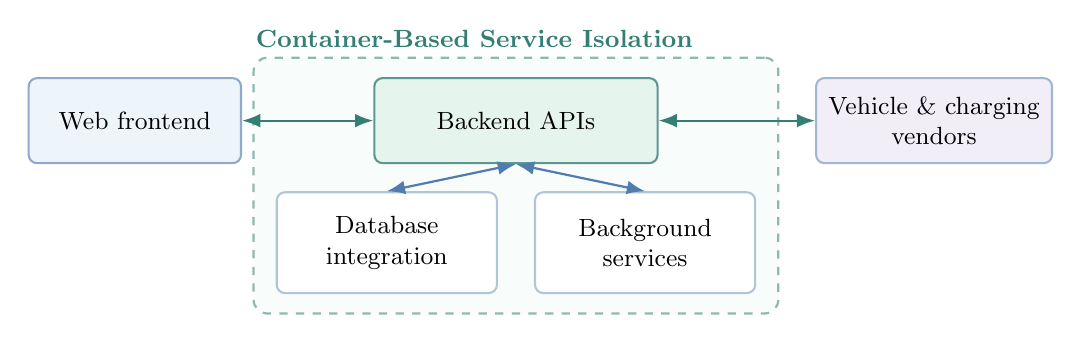
\begin{tikzpicture}[>=Latex]
    \node[fe] (ui) at (0,0) {Web frontend};
    \node[be] (api) at (4.84,0) {Backend APIs};
    \node[extbox] (vendor) at (10.15,0) {Vehicle \& charging\\vendors};
    \node[store] (db) at (3.20,-1.55) {Database\\integration};
    \node[store] (jobs) at (6.48,-1.55) {Background\\services};
    \begin{scope}[on background layer]
      \node[draw=Accent!55,dashed,fill=SoftMint!28,rounded corners=5pt,
        line width=0.8pt,inner xsep=8pt,inner ysep=7pt,
        fit={(api)(db)(jobs)}] (boundary) {};
    \end{scope}
    \node[anchor=south west,font=\small\bfseries,text=Accent,inner sep=1pt]
      at ([yshift=2pt]boundary.north west) {Container-Based Service Isolation};
    \draw[<->,Accent,thick] (ui) -- (api);
    \draw[<->,Accent,thick] (api) -- (vendor);
    \draw[<->,AccentBlue,thick] (api.south) -- (db.north);
    \draw[<->,AccentBlue,thick] (api.south) -- (jobs.north);
  \end{tikzpicture}\par}
  \vspace{0.25cm}
  {\small\bfseries\color{Accent}My contributions}\par\vspace{0.10cm}
  {\small System planning \& backend development\quad /\quad Database integration\par
  \vspace{0.08cm}Log analysis \& debugging\quad /\quad Deployment \& maintenance}
\end{frame}

% ============================================================
% SLIDE 4 - Personally developed simulator and representative scenarios
% ============================================================
\begin{frame}{NeoPower: Scenario-Based System Simulation}
  \takeaway{I developed a custom simulator for vendor interaction and failure reproduction.}
  \vspace{0.18cm}
  {\centering
  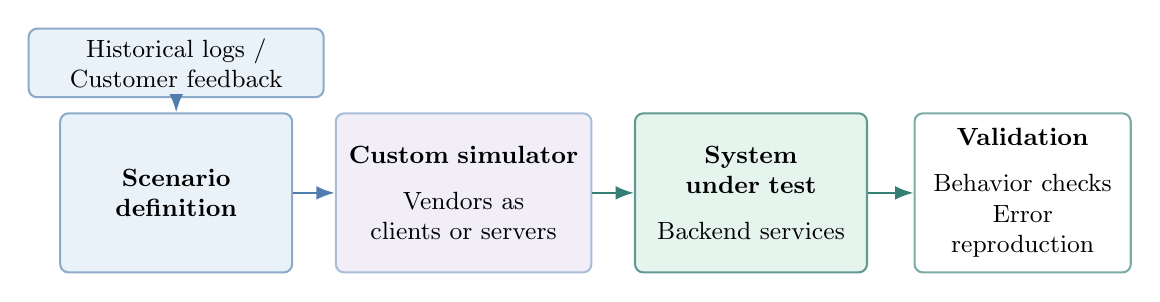
\begin{tikzpicture}[>=Latex]
    \node[scen,text width=3.5cm,minimum height=0.85cm,draw=AccentBlue!65,fill=SoftBlue] (history) at (0,1.65)
      {Historical logs /\\Customer feedback};
    \node[scen,text width=2.7cm,draw=AccentBlue!65,fill=SoftBlue] (def) at (0,0)
      {\textbf{Scenario}\\\textbf{definition}};
    \node[scen,text width=3.0cm,draw=AccentBlue!50,fill=SoftLilac] (sim) at (3.65,0)
      {\textbf{Custom simulator}\\[2mm]Vendors as\\clients or servers};
    \node[scen,text width=2.7cm,draw=Accent!78,fill=SoftMint] (sut) at (7.3,0)
      {\textbf{System under test}\\[2mm]Backend services};
    \node[scen,text width=2.5cm,draw=Accent!65,fill=white] (val) at (10.75,0)
      {\textbf{Validation}\\[2mm]Behavior checks\\Error reproduction};
    \draw[->,AccentBlue,thick] (history) -- (def);
    \draw[->,AccentBlue,thick] (def) -- (sim);
    \draw[->,Accent,thick] (sim) -- (sut);
    \draw[->,Accent,thick] (sut) -- (val);
  \end{tikzpicture}\par}
  \vspace{0.20cm}
  \begin{columns}[T,onlytextwidth]
    \begin{column}{0.486\textwidth}
      \begin{beamercolorbox}[rounded=true,sep=0.16cm,wd=\linewidth]{panelblue}
        {\small\bfseries\color{AccentBlue}High Load}\par\vspace{0.07cm}
        {\small Many buses arrive at once}
      \end{beamercolorbox}
    \end{column}
    \begin{column}{0.486\textwidth}
      \begin{beamercolorbox}[rounded=true,sep=0.16cm,wd=\linewidth]{panelmint}
        {\small\bfseries\color{Accent}Network Failure}\par\vspace{0.07cm}
        {\small Mass disconnection of stations / chargers}
      \end{beamercolorbox}
    \end{column}
  \end{columns}
\end{frame}

% ============================================================
% SLIDE 5 - Pre-deployment gate and operational algorithm comparison
% Cross-site comparisons are observational; caveat is in speaker notes.
% ============================================================
\begin{frame}{NeoPower: Testing \& Production Reliability}
  \begin{columns}[T,onlytextwidth]
    \begin{column}{0.40\textwidth}
      {\normalsize\bfseries\color{AccentBlue}Pre-Deployment Testing}\par
      \vspace{0.30cm}
      \centering
      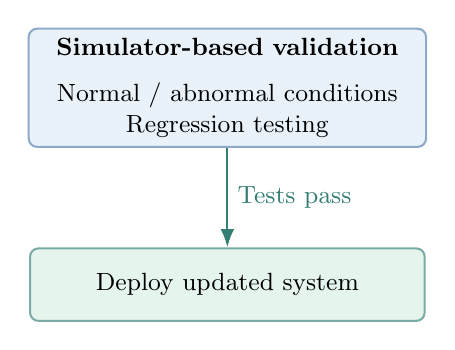
\begin{tikzpicture}[>=Latex]
        \node[scen,text width=4.8cm,minimum height=1.5cm,draw=AccentBlue!65,fill=SoftBlue] (test)
          {\textbf{Simulator-based validation}\\[2mm]Normal / abnormal conditions\\Regression testing};
        \node[flowstep,text width=4.8cm,fill=SoftMint] (deploy) at (0,-2.5) {Deploy updated system};
        \draw[->,thick,Accent] (test) -- node[right,font=\small] {Tests pass} (deploy);
      \end{tikzpicture}
    \end{column}
    \begin{column}{0.56\textwidth}
      {\normalsize\bfseries\color{Accent}Post-Deployment Validation}\par
      \vspace{0.30cm}
      {\small\bfseries Charging-power allocation algorithms}\par
      \vspace{0.18cm}
      {\small Cross-Site Comparison: similar operating conditions}\par
      \vspace{0.22cm}
      \centering
      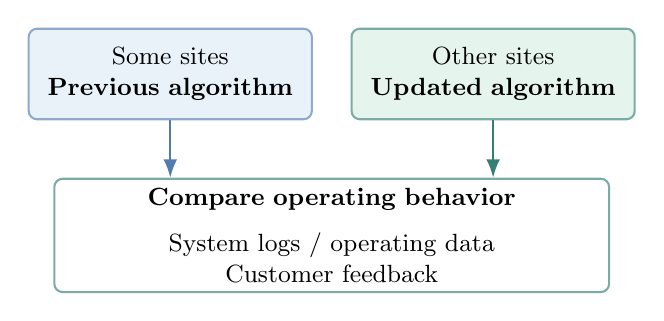
\begin{tikzpicture}[>=Latex]
        \node[scen,text width=3.35cm,minimum height=1.15cm,draw=AccentBlue!65,fill=SoftBlue] (old) at (0,0)
          {Some sites\\\textbf{Previous algorithm}};
        \node[scen,text width=3.35cm,minimum height=1.15cm,draw=Accent!65,fill=SoftMint] (new) at (4.1,0)
          {Other sites\\\textbf{Updated algorithm}};
        \node[scen,text width=6.8cm,minimum height=1.3cm,draw=Accent!65,fill=white] (data) at (2.05,-2.05)
          {\textbf{Compare operating behavior}\\[2mm]System logs / operating data\\Customer feedback};
        \draw[->,thick,AccentBlue] (old.south) -- (old.south |- data.north);
        \draw[->,thick,Accent] (new.south) -- (new.south |- data.north);
      \end{tikzpicture}
    \end{column}
  \end{columns}
\end{frame}

% Slide 6: Proposed A/E-centric architecture
\begingroup
\setbeamerfont{frametitle}{size=\fontsize{12}{14}\selectfont}
\begin{frame}{MoE Serving: HBM/HBF-Aware Attention--Expert Disaggregation}
  \takeaway{Co-design worker memory profiles and A/E placement to improve SLO goodput per watt.}
  \vspace{0.14cm}
  {\centering
  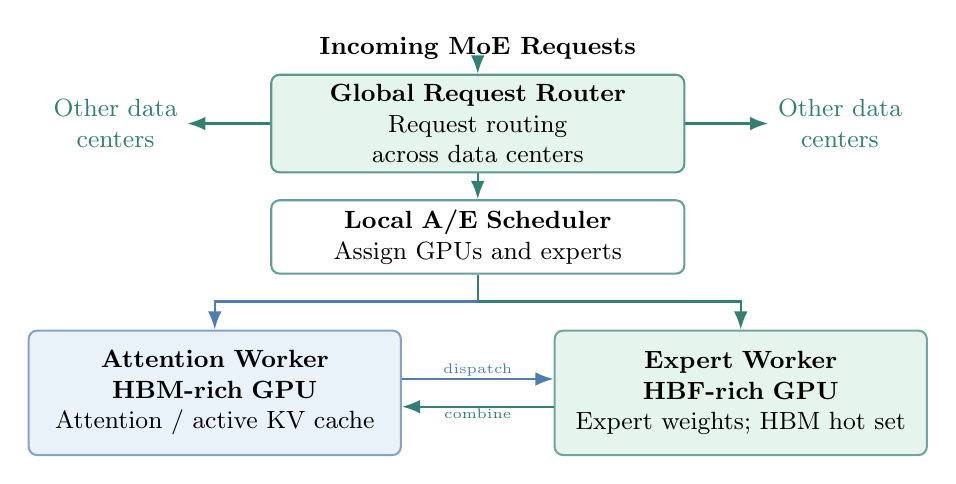
\begin{tikzpicture}[>=Latex]
    \node[font=\small\bfseries] (req) at (0,0.30) {Incoming MoE Requests};
    \node[svc,draw=Accent!80,fill=SoftMint,text width=5.0cm,minimum height=0.84cm]
      (global) at (0,-0.66) {\textbf{Global Request Router}\\Request routing across data centers};
    \node[svc,draw=Accent!75,fill=white,text width=5.0cm,minimum height=0.84cm]
      (local) at (0,-2.10) {\textbf{Local A/E Scheduler}\\Assign GPUs and experts};
    \node[align=center,font=\small,text=Accent] (dcLeft) at (-4.60,-0.66)
      {Other data\\centers};
    \node[align=center,font=\small,text=Accent] (dcRight) at (4.60,-0.66)
      {Other data\\centers};

    \node[svc,draw=AccentBlue!70,fill=SoftBlue,text width=4.48cm,minimum height=1.58cm]
      (attn) at (-3.34,-4.08) {\textbf{Attention Worker}\\\textbf{HBM-rich GPU}\\Attention / active KV cache};
    \node[svc,draw=Accent!70,fill=SoftMint,text width=4.48cm,minimum height=1.58cm]
      (expert) at (3.34,-4.08) {\textbf{Expert Worker}\\\textbf{HBF-rich GPU}\\Expert weights; HBM hot set};

    \draw[->,Accent,thick] (req) -- (global);
    \draw[->,Accent,thick] (global.west) -- (dcLeft.east);
    \draw[->,Accent,thick] (global.east) -- (dcRight.west);
    \draw[->,Accent,thick] (global) -- (local);
    \draw[Accent,thick] (local.south) -- (0,-2.92);
    \draw[->,AccentBlue,thick] (0,-2.92) -| (attn.north);
    \draw[->,Accent,thick] (0,-2.92) -| (expert.north);
    \draw[->,AccentBlue,thick]
      ([yshift=5pt]attn.east) -- node[above,font=\tiny,fill=white,inner sep=0.5pt] {dispatch}
      ([yshift=5pt]expert.west);
    \draw[->,Accent,thick]
      ([yshift=-5pt]expert.west) -- node[below,font=\tiny,fill=white,inner sep=0.5pt] {combine}
      ([yshift=-5pt]attn.east);
  \end{tikzpicture}\par}
  \vspace{0.12cm}
  {\centering\small\color{Accent}\textbf{Goal:} Balance trade-offs among latency, power, and throughput.\par}
\end{frame}
\endgroup

% ============================================================
% SLIDE 7 - System-level methodology; memory integration remains planned
% ============================================================
\begin{frame}{Research Methodology: System-Level Simulation}
  \takeaway{Model heterogeneous hardware to evaluate LLM serving scheduling.}
  \vspace{0.25cm}
  {\centering
  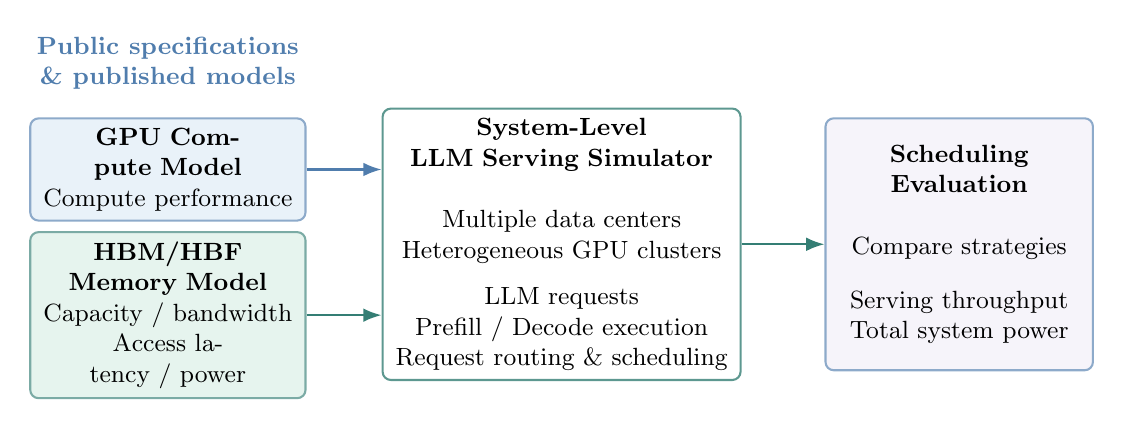
\begin{tikzpicture}[>=Latex]
    \node[align=center,font=\small\bfseries,text=AccentBlue] at (0,2.30)
      {Public specifications\\\& published models};
    \node[svc,draw=AccentBlue!65,fill=SoftBlue,text width=3.25cm,minimum height=1.05cm]
      (gpu) at (0,0.95) {\textbf{GPU Compute Model}\\Compute performance};
    \node[svc,draw=Accent!65,fill=SoftMint,text width=3.25cm,minimum height=1.35cm]
      (mem) at (0,-0.90) {\textbf{HBM/HBF Memory Model}\\Capacity / bandwidth\\Access latency / power};
    \node[svc,draw=Accent!80,fill=white,text width=4.3cm,minimum height=3.20cm]
      (sim) at (5,0) {\textbf{System-Level}\\\textbf{LLM Serving Simulator}\\[4mm]
      Multiple data centers\\Heterogeneous GPU clusters\\[2mm]
      LLM requests\\Prefill / Decode execution\\Request routing \& scheduling};
    \node[svc,draw=AccentBlue!65,fill=SoftLilac!65,text width=3.15cm,minimum height=3.20cm]
      (eval) at (10.05,0) {\textbf{Scheduling Evaluation}\\[4mm]
      Compare strategies\\[3mm]
      Serving throughput\\Total system power};
    \draw[->,AccentBlue,thick] (gpu.east) -- (sim.west |- gpu.east);
    \draw[->,Accent,thick] (mem.east) -- (sim.west |- mem.east);
    \draw[->,Accent,thick] (sim.east) -- (eval.west);
  \end{tikzpicture}\par}
  \vspace{0.33cm}
  {\small\color{Accent}\textbf{Architectural starting point:} open-source GPU-cluster serving simulator\par}
  \vspace{0.13cm}
  {\small\textbf{Planned integration:} published GPU-memory and storage-system models\par}
\end{frame}

% ============================================================
% SLIDE 8 - Close
% ============================================================
{\setbeamertemplate{footline}{}
\begin{frame}[plain]
  \vfill
  \begin{center}
    {\fontsize{38}{44}\selectfont\bfseries\color{Ink}Thank You}\par
    \vspace{0.30cm}
    {\Large\color{Accent}Questions \& Discussion}
  \end{center}
  \vfill
\end{frame}}

\end{document}
